\documentclass[10pt, conference]{IEEEtran}
\IEEEoverridecommandlockouts

\usepackage{cite}
\usepackage{amsmath,amssymb,amsfonts}
\usepackage{graphicx}
\usepackage{textcomp}
\usepackage{xcolor}
\usepackage{url}
\usepackage{booktabs}

% tighten float (figure/table) spacing to fit 2 pages
\setlength{\textfloatsep}{4pt plus 1pt minus 1pt}
\setlength{\floatsep}{4pt plus 1pt minus 1pt}
\setlength{\intextsep}{4pt plus 1pt minus 1pt}
\setlength{\dbltextfloatsep}{4pt plus 1pt minus 1pt}
\setlength{\abovecaptionskip}{2pt}
\setlength{\belowcaptionskip}{0pt}
% tighten space around displayed equations (distribution-robust margin)
\setlength{\abovedisplayskip}{3pt plus 1pt minus 1pt}
\setlength{\belowdisplayskip}{3pt plus 1pt minus 1pt}
\setlength{\abovedisplayshortskip}{1pt plus 1pt}
\setlength{\belowdisplayshortskip}{1pt plus 1pt}

\def\BibTeX{{\rm B\kern-.05em{\sc i\kern-.025em b}\kern-.08em
    T\kern-.1667em\lower.7ex\hbox{E}\kern-.125emX}}

\begin{document}

\title{Difficulty Analysis of Posiform-Planted QUBO Benchmarks via Energy and Hamming Metrics}

\author{
\IEEEauthorblockN{Yideun Kim}
\IEEEauthorblockA{
Department of Computer Engineering\\
Kangwon National University\\
Chuncheon, Republic of Korea\\
Email: rladlems1031@kangwon.ac.kr}
\and
\IEEEauthorblockN{Dongjae Lee$^{\dagger}$}
\IEEEauthorblockA{
Department of Convergence Security\\
Kangwon National University\\
Chuncheon, Republic of Korea\\
Email: dongjae.lee@kangwon.ac.kr}
\thanks{This work was supported in part by the Korea Internet \& Security Agency
(KISA) grant funded by the Korean government (Ministry of Science and ICT,
MSIT) through the ``Information Security Workforce Development (Information
Security Specialized University Program)'' in 2026 and in part by the Basic Science Research Program through the National Research
Foundation of Korea (NRF) funded by the Ministry of Education (No.~25411243).}
\thanks{$^{\dagger}$Corresponding author: Dongjae Lee.}
}

\maketitle

\begin{abstract}
Benchmarking QUBO solvers requires instances with a known optimum that stay hard.
Posiform planting builds such instances with a unique optimum. A recent variant
adds random spin-glass terms and scales the planted term by a coefficient
$\alpha$ to tune hardness. Prior work characterizes this hardness only
empirically, via the success rate, which shows that difficulty varies with the
parameters but not why, and cannot compare instances at $0\%$ success. We instead measure how close failing runs come to the optimum. Over
failures only, on a fixed hardest-instance set, we record the energy gap and
Hamming distance (HD) to the planted answer. These resolve the flat $0\%$ into a continuous difficulty curve with a clear
structure: $\Delta E = \Delta R + \alpha\Delta P$, a local-minimum floor plus a
growing planted penalty. Under simulated annealing (SA) on a D-Wave Pegasus
graph ($n{=}5612$) it is non-monotone in $\alpha$: $\Delta E$ peaks then declines
while HD falls throughout, with the peak where the rising penalty is overtaken
by failures drifting toward the optimum. A D-Wave Advantage run reproduces the
shape, suggesting an instance property, not SA alone.
Reporting both quantities grades planted QUBO benchmarks even when no run
succeeds.
\end{abstract}

\begin{IEEEkeywords}
QUBO benchmarking, posiform planting, quantum annealing,
simulated annealing, Hamming distance, energy gap, $\alpha$-difficulty.
\end{IEEEkeywords}

\section{Introduction}
Benchmarking quantum annealers and classical heuristics on QUBO problems needs
instances whose optima are known but hard to find. Posiform
planting~\cite{hahn2023posiform} produces QUBOs with a unique ground state, but
they are easy for simulated annealing (SA)~\cite{kirkpatrick1983}. Pelofske et
al.~\cite{pelofske2024hardened} made them harder. They add random
discrete-coefficient spin-glass QUBOs $R_i$ to a posiform-planted QUBO $P$ with
unique minimum $x^\star$, scaled by a coefficient $\alpha$:
\begin{equation}
  Q_{\alpha}(x) \;=\; \sum_{i} R_{i}(x) \;+\; \alpha\,P(x).
  \label{eq:qalpha}
\end{equation}
That study tuned hardness mainly through the random-QUBO size and the
annealing time. It fixed $\alpha\in\{0.01,0.1\}$ and reported the ground-state
success rate. But this rate is $0\%$ across the whole small-$\alpha$ regime. It
cannot rank instances, solvers, or $\alpha$ values. Pelofske et al.\ conjecture
that the hardness comes from local minima whose energy is very close to the true
ground state.

We make that conjecture quantitative. $\Delta E$ measures local-minimum depth.
But over all samples it mixes depth with the success rate. We therefore
condition on failure and use the $100$ hardest instances, held fixed as $\alpha$
varies. Measured this way, failure-conditioned $\Delta E$ and Hamming distance
(HD) reveal a $\Delta R{+}\alpha\Delta P$ structure with a non-monotone peak.
Neither quantity is new. Our contribution is the protocol. Failure-conditioning
on a fixed hardest set turns the uninformative $0\%$ rate into a rankable curve.
A supporting quantum-annealer run is consistent with this structure coming from the instances, not SA alone.

\section{Methodology}
\textbf{Instances.} We generate $500$ posiform-planted instances on the D-Wave
Pegasus P16 graph~\cite{boothby2020} ($n{=}5612$ qubits). Each coefficient
$R_{ij}$ is $-1$ or $+1$. We split the graph into blocks of at most $16$ qubits
by recursive bisection and solve each block $R_i$ exactly. The planted target
$x^\star$ is the concatenation of the block ground states, so it is the global
minimum of $\sum_i R_i$. $P$ is the posiform of a planted 2-SAT whose only
solution is $x^\star$. We rank the $500$ instances by their total SA
failing-reads across the sweep and fix the hardest $100$ as a constant set. This
set is chosen from SA alone, before any QPU run, so the cross-solver agreement
is not circular. We then run both solvers on it.

\textbf{Metrics.} For each sample $x$ we record HD$(x,x^\star)$~\cite{hamming1950}
and the energy gap $\Delta E = E(x)-E(x^\star)\geq 0$ under the same $Q_\alpha$.
Because every $R_{ij}$ is $\pm1$, each $R$ energy is an integer. We therefore
report $\Delta E$ in units of the smallest non-degenerate $R$ gap
($\Delta_R{=}1$). This unit is the same across instances, as is HD$/n$. A read counts
as a success only when it equals $x^\star$ (a bit match), so the $0\%$ success
rate and the per-read failure rate both track $x^\star$ exactly. This differs
from matching the ground-state energy, which at $\alpha{=}0$ is degenerate
(Sec.~\ref{sec:vpc}).
At large $\alpha$, correct samples ($\Delta E{\approx}0$, HD${=}0$) drive both
quantities to $0$. We therefore condition all statistics below on failure
($x{\neq}x^\star$). Means are over failing reads. The instance-level standard
error stays below $0.06\,\Delta_R$, so we omit error bars.

\textbf{Protocol.} We sweep $\alpha$ over $0$, $10^{-9}$, $10^{-5}$, $10^{-4}$,
$10^{-3}$, $3{\times}10^{-3}$, $5{\times}10^{-3}$, $10^{-2}$, $1.5{\times}10^{-2}$,
and $2{\times}10^{-2}$. Beyond $2{\times}10^{-2}$
the instances are increasingly solved, so no fixed failing set remains. The main
sweep uses the \texttt{neal} SA package~\cite{neal} at $1000$ sweeps and $100$
reads per (instance,\,$\alpha$); we also run a separate $150$-instance subset
(not the hardest-$100$) at $1000$ and $5000$ sweeps to compare budgets. For a
cross-solver check we replay the same
$100$ instances on a D-Wave Advantage annealer (\texttt{Advantage\_system6.4}).
The run is hardware-native, with auto-scaling, two-gauge averaging, and $100$
reads at $20\,\mu$s. We recompute $\Delta E$ from $Q_\alpha$.

\section{Results}

\begin{figure}[!t]
\centering
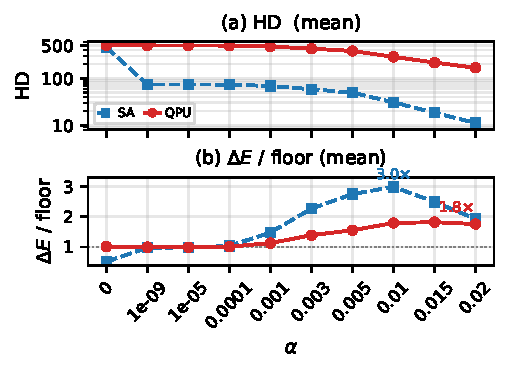
\includegraphics[width=0.82\columnwidth]{figures/fig_sa_vs_qpu.pdf}
\caption{Failure-conditioned difficulty over the $100$ hardest instances. At
each $\alpha$, at least $91\%$ of reads fail. Blue: SA. Red: a D-Wave Advantage
annealer. (a)~HD on a log axis falls monotonically but never reaches $0$.
(b)~$\Delta E$ rescaled by each solver's small-$\alpha$ floor (SA
$\approx1.1\,\Delta_R$, QPU $\approx24$), on one axis. Both start at $1$. SA
rises to a peak of $3.0\times$ near $\alpha{=}10^{-2}$, then declines. The
annealer shows the same shape but more weakly ($1.8\times$).}
\label{fig:traj}
\end{figure}

\subsection{Floor, peak, and decline of $\Delta E$}
\label{sec:vpc}
At $\alpha{=}0$ the random part $R$ is degenerate. Here $56.1\%$ of samples
reach an $R$ ground state ($\Delta E{=}0$), yet $0\%$ equal $x^\star$, and HD is
maximal ($459$, or $8.2\%$ of $n$). So $\Delta E$ alone would read as solved,
but HD shows no sample is near $x^\star$. For $\alpha{>}0$ (Fig.~\ref{fig:traj}b),
in the small-$\alpha$ region ($\alpha\in[10^{-9},10^{-4}]$), $\alpha\Delta P$ is
negligible and $\Delta E$ stays flat at the depth of a local-minimum trap in $R$. We call this
flat value the floor (mean $1.10$, median $1$). This floor of $\approx1\,\Delta_R$
is the quantitative content of the local-minimum conjecture
in~\cite{pelofske2024hardened}: in the small-$\alpha$ limit, failing samples sit
about one $R$-gap above $x^\star$. HD is also flat ($\approx73$). Past $\alpha{=}10^{-3}$ the planted term grows. $\Delta
E$ rises to a peak of $3.35$ at $\alpha{=}10^{-2}$, which is $3.0\times$ the
floor, then declines to $2.16$. The floor, peak, and decline are separated by
far more than the instance-level SE ($<0.06\,\Delta_R$). HD meanwhile falls
monotonically ($73\to11$). So failing samples move closer to $x^\star$ in bits
even as their energy gap grows. The peak comes from a
competition. For a fixed failing bitstring,
$\Delta E{=}\Delta R{+}\alpha\Delta P$ is linear in $\alpha$ ($\Delta R,\Delta P$
fixed per bitstring). But the failing set is not fixed: as $\alpha$ rises,
failing samples drift toward $x^\star$ (HD falls), where $\Delta P$ is smaller.
The observed mean is an envelope over this moving population: it climbs while
$\alpha\Delta P$ dominates, then falls as the drift into smaller-$\Delta P$
regions wins. The peak is
not a survivorship or selection artifact. The $100$ instances fail at least
$91\%$ of reads at every $\alpha$ ($0\%$ ground-state success, as
\cite{pelofske2024hardened} report). The same shape appears over all $500$
instances (floor $\approx1.1$, peak $\approx3.0$), and the hardest set only
sharpens it.

\subsection{Quantum-annealer consistency check}
\label{sec:qpu}
As supporting evidence, we ran the same $100$ instances once on a D-Wave
Advantage annealer (Fig.~\ref{fig:traj}, red). It shows the same pattern. There
is $0\%$ success, a non-monotone $\Delta E$ peak near $\alpha{=}10^{-2}$, and a
monotonic HD decrease ($501\to167$). Its baselines sit an order of magnitude
above SA's ($\Delta E\approx24$, HD$\approx500$), and its peak is weaker in
relative terms ($1.8\times$ its floor versus SA's $3.0\times$). One run cannot
establish generality. But it is consistent with the structure being a property
of the instances, not of SA. The integrated control error (ICE) is the
annealer's control-precision limit: couplers carry a roughly fixed error of
order $0.02$--$0.03$. At the peak the planted couplers map to Ising
$J\approx0.03$, comparable to ICE, so the device only partly resolves the
signal, consistent with the weaker peak above. A smaller scale would push them
below ICE and should flatten it, which we leave to future work.

\section{Discussion and Conclusion}
Failure-conditioned $\Delta E$ measures difficulty (local-minimum depth) and
HD measures proximity to $x^\star$. Reporting both separates how deep a failure
is from how close it is. The all-sample mean (the success rate) hides the peak.
It falls at larger $\alpha$ only because more reads succeed, not because failures
are shallower. $\Delta E$ also separates solvers that the
success rate cannot: on the $150$-instance subset at $\alpha{=}10^{-3}$, both
budgets give $0\%$ success, yet $\Delta E$ is $1.68$ versus $1.00$. We therefore recommend
reporting failure-conditioned $\Delta E$ (floor and peak) with HD over a fixed
hardest set whenever an $\alpha$-like parameter is swept. This gives a
failure-conditioned diagnostic of the benchmark instances rather than a single
difficulty score. Absolute values still depend on the solver and schedule.

\textbf{Limitations.} The QPU evidence is a single run (two gauges, one
$20\,\mu$s anneal). The classical side is a single SA family. The instances use
one coefficient type ($\pm1$) and one topology (Pegasus).

\textbf{Future work:} broader classical solvers, more annealer gauges and
anneal times, other coefficient types and topologies, and joint
HD--$\Delta E$ analysis. Code and instances:
\url{https://github.com/YIDEUNKIM/qubo_dataset}.

\bibliographystyle{IEEEtran}
\begin{thebibliography}{99}
\scriptsize\setlength{\itemsep}{0pt}

\bibitem{hahn2023posiform}
G.~Hahn, E.~Pelofske, and H.~N.~Djidjev,
``Posiform planting: generating QUBO instances for benchmarking,''
\emph{Frontiers in Computer Science}, vol.~5, Art.~no.~1275948, 2023.

\bibitem{kirkpatrick1983}
S.~Kirkpatrick, C.~D.~Gelatt~Jr., and M.~P.~Vecchi,
``Optimization by simulated annealing,''
\emph{Science}, vol.~220, no.~4598, pp.~671--680, 1983.

\bibitem{pelofske2024hardened}
E.~Pelofske, G.~Hahn, and H.~N.~Djidjev,
``Increasing the hardness of posiform planting using random QUBOs for programmable quantum annealer benchmarking,''
\emph{npj Unconventional Computing}, vol.~2, Art.~no.~17, 2025.

\bibitem{boothby2020}
K.~Boothby, P.~Bunyk, J.~Raymond, and A.~Roy,
``Next-generation topology of D-Wave quantum processors,''
arXiv:2003.00133, 2020.

\bibitem{hamming1950}
R.~W.~Hamming, ``Error detecting and error correcting codes,''
\emph{Bell Syst. Tech. J.}, vol.~29, no.~2, pp.~147--160, 1950.

\bibitem{neal}
D-Wave Systems Inc., ``dwave-neal: a simulated annealing sampler,'' GitHub,
2022. \url{https://github.com/dwavesystems/dwave-neal}.

\end{thebibliography}

\end{document}
